%% 2019 07 04 Ph. G. Freimann
%%

\section{Wachstum und Zerfall}\index{Wachstum}\index{Zerfall}
\sectuntertitel{Sagt ein großer Stift zum kleinen Stift: ``Wachsmalstift!''}

%%%%%%%%%%%%%%%%%%%%%%%%%%%%%%%%%%%%%%%%%%%%%%%%%%%%%%%%%%%%%%%%%%%%%%%%%%%%%%%%%

\TRAINER{
  Video \href{https://www.youtube.com/watch?v=TMaLuks8dxw}{MatheMann}
Wo schneiden sich $x^3$ und $\e^x$?}%%
\subsection*{Lernziele}

\begin{itemize}
\item Zinseszins
\item Wachstums-, Zerfallsprozesse
\item Verdoppelungs- und Halbwertszeiten
%%\item Basiswechsel
\end{itemize}

\TadBMTA{342}{20}
%%\TALS{(\cite{frommenwiler17alg} S.221 (Kap. Exponentielles Wachstum))}
%%\TALS{(\cite{frommenwiler17alg} S.223 (Kap. Exponentielle Abnahme))}
%%\TALS{(\cite{frommenwiler17alg} S.225 (Kap. Zinseszins))}
%%\GESO{(\cite{marthaler21alg}       S.342 (Kap. 20))}

\newpage


\subsection{Beispiele}
Bei Wachstumsprozessen sprechen wir dann von einer exponentiellen
Zunahme, wenn die Zunahme pro Zeiteinheit immer proportional zum aktuellen Bestand ist.

\begin{itemize}
\item \Lueckentext{Zinseszins}
\item \Lueckentext{Frequenzen in der temperierten Stimmung
  (Musik). Zunahme der Frequenz pro Halbtonschritt.}
\item \Lueckentext{Keime in der Kuhmilch; ansteckungsbedingte Krankheitsfälle (\zB viral)}
\item \Lueckentext{Algenbefall in Teichen}
\item \Lueckentext{Generell Populationen: Flechten, Pilze}
\item \Lueckentext{(ungebremstes) Bevölkerungswachstum / bzw. Tierpopulation}
\item \Lueckentext{\dotfill}
\end{itemize}


\GESO{\olatLinkArbeitsblatt{Exponentialfunktionen}{https://olat.bms-w.ch/auth/RepositoryEntry/6029794/CourseNode/106029175831971}{Kap. 1.1:
    Voraussetzungen: Aufgaben 1. bis 3.}}
\TALS{\olatLinkArbeitsblatt{Exponentialfunktionen}{https://olat.bms-w.ch/auth/RepositoryEntry/6029786/CourseNode/106029175777725}{Kap. 1.1:
    Voraussetzungen: Aufgaben 1. bis 3.}}


\newpage

\subsection{Einstiegsbeispiel Taschengeld}

Bei Familie Cash kann man aussuchen, wie sich sein Taschengeld über
die Jahre «vermehrt». Mani wählt Variante A. Bei Variante A erhält man
CHF 1.- im ersten Jahr, CHF 2.- im 2. Jahr, CHF 3.- im 3. Jahr und so
weiter bis zur abgeschlossenen Grundbildung im 13. Jahr CHF 13.-.

Carla wählt Variante B. Bei der Variante B erhält Carla auch CHF 1.-
im ersten Jahr, dann aber jedes Jahr 30\% mehr, als im Vorjahr.

a) Wird Carla vor Ende der Grundbildung jemals mehr als Mani erhalten?

\LoesungsRaumLang{Ja, im 10. Schuljahr}

b) Skizzieren Sie beide Varianten ins untenstehende Koordinatensystem.

c) (challenge) Wer hat über alle Jahre in der Summe mehr Taschengeld?

\LoesungsRaumLang{Carla wird mehr haben}


\TRAINER{\bbwCenterGraphic{13cm}{allg/funktionen/img/taschengeldAusgefuellt.png}}
\noTRAINER{\bbwCenterGraphic{16cm}{allg/funktionen/img/taschengeld.png}}

\TRAINER{Optional: Zeige mit Geogebra (\texttt{geogebra.org}) $x^2$ vs. $1.4^x$. Fazit:
  Exponentielles Wachstum überholt jegliche Potenzfunktion. Bei
  ca. $x\approx 16.7541$ $y\approx 280.7$}
\newpage

\subsubsection{Grundform Wachstumsprozesse} \index{Exponentieller Prozess! Grundform}

\begin{definition}{Wachstum}{}\index{Wachstum|textbf}
  Die Grundform des exponentiellen Wachstums wird beschrieben durch die Funktion
$$f(x): x \mapsto a^x$$
  bzw.
  $$y = a^x$$
\end{definition}

\subsubsection*{Aufgaben}
\GESO{\olatLinkArbeitsblatt{Exponentialfunktionen}{https://olat.bms-w.ch/auth/RepositoryEntry/6029794/CourseNode/106029175831971}{Kap. 1.2:
    Einfache Wachstumsprozesse: Aufgaben 4. bis 6.}}
\TALS{\olatLinkArbeitsblatt{Exponentialfunktionen}{https://olat.bms-w.ch/auth/RepositoryEntry/6029786/CourseNode/106029175777725}{Kap. 1.2:
    Einfache Wachstumsprozesse: Aufgaben 4. bis 6.}}


\newpage


\subsection{Exponentieller Zerfall}\label{zerfallsfunktion}


\subsubsection{Beispiele}
\begin{itemize}
	\item \Lueckentext{Zinsliche Abschreibungen (\zB Wert eines Autos)}
	\item \Lueckentext{Radioaktiver Zerfall}
	\item \Lueckentext{Lichtintensität in Medium (Gas / Flüssigkeit / Glasfaser), dies gilt vertikal, wie auch horizontal}
	\item \Lueckentext{Atmosphärischer Luftdruck in Metern über Meer}
  \item \Lueckentext{Entladen einer Batterie bzw. eines Kondensators}
  \item \Lueckentext{Sauerstoffkonzentration in Seen (\zB Herbst bei kontinuierlicher Abnahme)}
  \item \Lueckentext{Abnahme des Bierschaums im Glas}
  \item \Lueckentext{Mischen, wie im Sirup-Beispiel\totalref{sirup_beispiel}}
  \item \Lueckentext{«Halbwertszeit des Wissens» ;-)}
  \item \Lueckentext{\dotfill}
\end{itemize}

\newpage

Die Funktion $f(x): x \mapsto y = d^{-x}$ ist eine
Exponentialfunktion, die gegen Null geht.

\bbwFunction{-4}{4}{-1}{8}{exp(-\x)}{-2:4}
\newpage

\subsubsection{Grundform Zerfallsprozesse} \index{Exponentieller Prozess! Grundform}
Die Grundform für Zerfallsprozesse lautet:

\begin{definition}{Zerfall}{}\index{Zerfall|textbf}
  Die Grundform des exponentiellen Zerfalls wird beschrieben durch die Funktion
$$f(x): x \mapsto a^x$$
  bzw.
  $$y = a^x$$
\end{definition}


\begin{gesetz}{Wachstum vs. Zerfall}{}

  Der einzige Unterschied bei Wachstums- bzw Zerfallsprozessen ist der
  Faktor $a$:

  \begin{itemize}
    \item \LoesungsRaumLen{40mm}{$a>1$: Wachstum}\vspace{3mm}
    \item \LoesungsRaumLen{40mm}{$0<a<1$: Zerfall}
  \end{itemize}
  
\end{gesetz}


\begin{bemerkung}{$x$-Richtung}{}
  Exponentielle Prozesse laufen meist in der Zeit ab. Somit wird
  die $x$-Achse zur Zeitachse und meist mit $t$ (Time) bezeichnet:
  $$f(t) = a^t$$
  \end{bemerkung}


\subsection*{Aufgaben}
%%\TALSAadBMTA{223ff}{840., 841., 843., 844. und 846.}

\GESO{\olatLinkArbeitsblatt{Exponentialfunktionen}{https://olat.bms-w.ch/auth/RepositoryEntry/6029794/CourseNode/106029175831971}{Kap. 1.3: Zerfall: Aufg. 7., 8. und 9.}}
\TALS{\olatLinkArbeitsblatt{Exponentialfunktionen}{https://olat.bms-w.ch/auth/RepositoryEntry/6029786/CourseNode/106029175777725}{Kap. 1.3: Zerfall: Aufg. 7. 8. und 9.}}

\TRAINER{ev. hier Beispiel «Sirup» aus dem Anhang}

\AadBMTA{354}{9. (Bauchspeicheldrüse)}
\olatLinkGESOKompendium{3.4.1}{27ff}{33., 35., 36., 39. und 41.}

%\newpage
%%% Sirup-Beispiel
\subsection{Mischtank}\index{Mischtank}\index{Sirup}\label{sirup_beispiel}
Wird ein Glas Wasser in ein Glas Sirup geschüttet, so

\TRAINER{\bbwCenterGraphic{5cm}{allg/alg/potenzen_wurzeln/img/Schwapp.png}}%%
\noTRAINER{\bbwCenterGraphic{5cm}{allg/alg/potenzen_wurzeln/img/SchwappOhneFormel.png}}

geschieht erst mal etwas eher klebriges:
\begin{itemize}
  \item Das Wasser verdrängt den Sirup und
  \item das Sirupglas schwappt über.
\end{itemize}

Wenn man nun gleichzeitig im Sirupglas
umrührt, so mischt sich das Wasser mit dem Sirup und je länger man
Wasser einschüttet, umso verdünnter wird der Sirup.


Wie viel Sirup bleibt im Glas?

\TNT{2.4}{
Am Ende bleibt ein
Verhältnis von Wasser : Sirup = $\left(1-\frac{1}{e}\right) : \left(\frac{1}{e}\right)$
\vspace{1.5cm}
}

Diese Konstante wird oft in großen chemischen Mischtanks verwendet,
gibt aber auch ein Maß an, wenn \zB in einer Minergie-Wohnung die Luft
ausgetauscht wird. Wenn nämlich das Volumen der Wohnung einmal neu hineingepumpt (bzw. weggeblasen) wurde während sich alte die Luft im Haus permanent mit der neuen vermischt, so ist noch ein Anteil von \TRAINER{$\frac{1}{e}$}\noTRAINER{ ..... } der alten Luft im Haus.
\newpage


\textbf{Begründung:}\\
1. Gedanke: Jedes eingefüllte Glas, vermindert die vorhandene
Sirupkonzentration um den selben Faktor. Ergo handelt es sich um
einen exponentiellen Zerfall.

\leserluft

2. Gedanke: Wir tauschen drei Mal $\frac13$ aus. Nehmen also im
\begin{itemize}
\item \textbf{ersten Schritt} $\frac13$ des Sirups weg (und ersetzen diesen mit Wasser).
  Es bleiben $\frac23$ Sirup. Den Rest füllen wir mit Wasser auf.
\item Im \textbf{zweiten Schritt} nehmen wir $\frac13$ des Gemisches
weg; es verbleiben also $\frac23$ von $\frac23$ an
Sirup-Konzentrat. Der Rest wird immer wieder mit Wasser aufgefüllt. Mit
anderen Worten: Es bleiben $\frac23 \cdot \frac23
= \left(\frac23\right)^2$ an Sirup\footnote{Man könnte hier auch argumentieren mit: «Wir nehmen von den $\frac23$ einen Drittel weg»: $\frac23 - (\frac13$ von $\frac23)$ = $\frac23 - (\frac13 \cdot\frac23) = \frac23 \cdot(1-\frac13)=\frac23\cdot\frac23$}.
\item Im \textbf{dritten Schritt} entnehmen wir wieder $\frac13$ des
Gemisches; es verbleiben wieder $\frac23$ vom bisherigen Sirup, also
$\frac23$ von $(\frac23)^2$ also $\left(\frac23\right)^3$.

Beim dreistufigen Gedankenexperiment verbleiben
$\left(\frac23\right)^3 = \left(1-\frac13\right)^3$ der ursprünglichen Konzentration.
\end{itemize}
\leserluft

3. Gedanke: Das Experiment vom vorherigen Gedanken können wir natürlich auch mit immer kleineren\TALS{, sogenannten infinitesimalen,} Schritten durchführen.
Mit Centilitern \zB im dl-Glas ersetzen wir 10 Mal je $\frac1{10}$. 
So verbleibt am Schluss $\left(1-\frac{1}{10}\right)^{10}\approx 0.35$ Sirup.

\GESO{Wenn wir (\zB mit dem Taschenrechner) die Schrittanzahl immer weiter vergrößern (und somit die pro Schritt ausgetauschte Menge immer verkleinern), so ergibt sich für 1000 Schritte ein Verhältnis von $\left(1-\frac{1}{1000}\right)^{1000}\approx 0.3677 \approx \frac1{\e}$. }
\TALS{Wenn wir die Schritte permanent erhöhen (und gegen Unendlich gehen lassen), so erhalten wir den Grenzwert (lat. Limes) von

$$\lim_{n\rightarrow\infty} \left(1-\frac{1}{n}\right)^n = \frac1{\e}$$
}
\newpage

\textbf{Aufgabe 1: Sirup}\\
Wie viel Wasser muss eingeschüttet werden, damit das auf der Flasche
angegebene Verhältnis von 1:6 (1 Teil Sirup, 6 Teile Wasser) zustande
kommt?

\TNT{8}{
Bei 1x Schütten, erhalten wir $\left(\frac{1}{\e}\right)^1$ Anteil Sirup.

Bei 2x Schütten, erhalten wir $\left(\frac{1}{\e}\right)^2$ Anteil Sirup.

Somit erhalten wir den Siebtel (1:6 = $\frac17$-Anteil) indem wir die
folgende Exponentialgleichung lösen:

$$\frac17 = \left(\frac{1}{\e}\right)^n$$
Diese Gleichung lösen wir, indem wir beidseitig logarithmieren und so
erhalten wir den einzuschüttenden Teil $$n=\ln(7)\approx{1.946}.$$
}%% END TNT

\textbf{Aufgabe 2: Minerige-Haus}\\
Wenn wir also wissen wollen, wie viel Luft in ein Minergiehaus
eingepumpt werden muss, damit nur noch 1 Promille der alten Luft
vorhanden ist, so erhalten wir
\TNTeop{
  $$\text{Volumen Neuluft} = \text{Wohnungsvolumen}\cdot{}\ln(1000)$$
  $$\ln(10000) \approx 6.9$$
} %% end TNT


\newpage

\newpage


\subsection{Startwert}\index{Startwerte!bei Wachstums- und Zerfallsprozessen}

Die bisher betrachteten Exponentialfunktionen haben für den Wert $x=0$ (bzw. $t=0$) immer den
$y$-Wert = 1 bzw. 100\%.
Da in der Praxis meist konkrete Werte vorgegeben sind verwenden wir
eine \textbf{allgemeinere Form der Exponentialfunktion}.

\subsubsection{Einstiegsbeispiel}

\begin{beispiel}{Pilz}{}
  Ein Pilzbefall an einer Wand nehme täglich um 23\% der Fläche
  zu\footnote{Je nach Organismus ist auch ein quadratisches Wachstum
  vorhanden, doch für unser Experiment verwenden wir exponentielles Wachstum.}.
  Anfänglich wird eine Fläche von $35$ $\text{cm}^2$ gemessen.
  Welche Fläche ist nach einem, nach zwei, nach fünf, nach zehn
  bzw. nach $n$ 
  Tagen zu erwarten?

  \TNT{6}{Ein  Tag:   $35\cdot{} 1.23^1    =          43.05 \text{cm}^2$\\
          Zwei Tage:  $35\cdot{} 1.23^2   \approx{}  52.95 \text{cm}^2$\\
          Fünf Tage:  $35\cdot{} 1.23^5   \approx{}  98.54 \text{cm}^2$\\
          Zehn Tage:  $35\cdot{} 1.23^{10} \approx{} 277.4 \text{cm}^2$\\
          $n$  Tage:  $35\cdot{} 1.23^n = 35\cdot{}1.23^n$}%% END TNT

  Wann wird die ganze Wand ($6 \text{ m}^2$) mit dem Pilz befallen
  sein?
  
\TNT{6}{$6 \text{ m}^2 = 60\,000 \text{ cm}^2$
     
     ergo: $60\,000 = 35 \cdot{} 1.23^n$

     (durch 35 teilen, dann logarithmieren)

     $$\frac{60\,000}{35} = 1.23^n$$

     $$n = \log_{1.23}\left(\frac{60\,000}{35}\right) \approx 35.97 \text{Tage}$$

   }%% END TNT

\end{beispiel}

\newpage


\begin{gesetz}{Exponentialfunktion mit frei wählbarem Startwert}{}
$$f: y = \LoesungsRaumLen{40mm}{b\cdot{}a^x}$$

Auch hier gibt der Parameter $a$ den Wachstumsfaktor pro Zeiteinheit $e_x$ an.

Dabei ist $b$ der Startwert zum Zeitpunkt $x$ = 0.
\end{gesetz}


\noTRAINER{\bbwCenterGraphic{8cm}{allg/funktionen/img/exp/b_faktor.png}}
\TRAINER{\bbwCenterGraphic{8cm}{allg/funktionen/img/exp/b_faktor_trainer.png}}

\begin{bemerkung}{Wachstumsfaktor}{}{}
Werden zwei $x$ Positionen mit Differenz 1 (=$e_x$) betrachtet, so sind
die zugehörige $y$-Werte um \textbf{Faktor} $a$ auseinander.
\end{bemerkung}

Begründung:
\TNTeop{
  Gegeben $x_1$ und $x_2 = x_1 + 1$. So ist

  $y_1 = b\cdot{}a^{x_1}$ und $y_2 = b\cdot{}a^{x_2}$.

  Setzen wir nun $x_1 + 1$ für $x_2$ ein, so erhalten wir:

  $$y_2 = f(x_2) = b\cdot{}a^{x_2} = b\cdot{} a^{x_1+1} =  b\cdot{}a^{x_1} \cdot{} a^1 = y_1\cdotp{} a$$
}
\newpage


\subsection*{Aufgaben}

\GESO{\olatLinkArbeitsblatt{Exponentialfunktionen}{https://olat.bms-w.ch/auth/RepositoryEntry/6029794/CourseNode/106029175831971}{Kap. 1.4:
    Frei wählbarer Startwert: Aufg. 10. Gummiball; 11. Neophytenplage;
    12: Tierpopulation; 13. Licht im Wasser;  weitere Aufgaben 14. bis 17.}}
\TALS{\olatLinkArbeitsblatt{Exponentialfunktionen}{https://olat.bms-w.ch/auth/RepositoryEntry/6029786/CourseNode/106029175777725}{Kap. 1.4:
    Frei wählbarer Startwert: Aufg. 10. Gummiball; 13. Licht im Wasser. 14. Federpendel; 15. Luftdruck; weitere Aufgaben aus
    Kap. 1.4.}}
 
  \AadBMTA{338}{29. (Bierschaum)}
  \AadBMTA{353}{6. (C-14 Methode)}

  Als Vorbereitung zur allgemeinen Wachstumsfunktion:
  \AadBMTA{207}{10. (Algen)}

\newpage


\subsection{Beobachtungszeitspanne}
\subsubsection{Einstiegsbeispiel}
\bbwCenterGraphic{17cm}{allg/funktionen/img/tuerlersee2.jpg}
\begin{center}{\small Legende: Türlersee April 2022}\end{center}

Der Türlersee ist ein kleiner See im Reppischtal. Seine Oberfläche
begann sich vor einigen Jahrzehnten stark mit Algen\footnote{Genau
  genommen handelte es sich um Zooplanktonbiomasse zwischen 1982 und 1994, doch als
  Idee zur Exponentialfunktion sollte ein ungefähres Flächenmodell reichen.} zu bedecken.

Anfänglich (zum Zeitpunkt $t=0$) waren gerade mal $20 \text{ m}^2$ bedeckt. Doch nach fünf Tagen hatte sich diese Fläche verdoppelt und nach weiteren fünf Tagen nochmals verdoppelt (also insgesamt vervierfacht).

Füllen Sie die (prognostizierte) Wertetabelle für 30 Tage ein:

\def\spaceX{\,\,\,\,\,\,\,\,\,\,}
\newcommand\tuerlerB[1]{\noTRAINER{\spaceX}\TRAINER{#1}}
\begin{tabular}{l|c|c|c|c|c|c|c}
  $t$:  & 0 & 5 & 10 & 15 & 20 & 25 & 30 \\
  \hline
  $m^2$ & \tuerlerB{20}  & \tuerlerB{40}  &   \tuerlerB{80}  &  \tuerlerB{160}  &  \tuerlerB{320}  &  \tuerlerB{640}  &  \tuerlerB{1280} \\
\end{tabular}

\newpage
Zeichnen Sie die Algenpopulation als Graph in eine Koordinatensystem
(beginnen Sie mit dem Ursprung ganz links unten. $x$-Achse in Tagen ($t$). $y$-Achse in $\text{m}^2$.

\noTRAINER{\bbwCenterGraphic{170mm}{allg/funktionen/img/exp/WachstumTuerlerseeLeer.png}}
\TRAINER{\bbwCenterGraphic{150mm}{allg/funktionen/img/exp/tuerlerAlgen.png}}

\TRAINER{In Graphik die Skala $t=$ Tage und $y=\text{m}^2$ noch eintragen.}

\TALS{challenge: Wie lautet die zugehörige Funktionsgleichung?

$$y = f(t) = \LoesungsRaumLen{40mm}{20\cdot{}2^{\frac{t}5}}$$}

\newpage



\textbf{Funktionsgleichung}

Wir betrachten nochmals diese Algenpopulation mit einer
Ver\textbf{\color{blue}dopplung} der Fläche alle \textbf{\color{red}fünf} Tage bei einer
Startfläche von \textbf{\color{green}zwanzig} $\text{m}^2$.

Geben Sie eine Funktionsgleichung an, welche das Wachstum der
Algenpopulation beschreibt...



\begin{bbwFillInTabular}{c|c|c||c|c|c|c|c|c|c|c}\hline
  Tage      & $t$ & \cellcolor{gray!75}\noTRAINER{\hspace{2cm}} & 0            & \tiny{1-4} & 5            & \tiny{6-9} & 10           & \tiny{11-14} & 15           &\\\hline
  Fläche     & $A$ & \TRAINER{$20\cdot v$}    &
  \TRAINER{20}\noTRAINER{\hspace{15mm}} &  \cellcolor{gray!75}    &
  \TRAINER{40}\noTRAINER{\hspace{15mm}} &    \cellcolor{gray!75}  &
  \TRAINER{80}\noTRAINER{\hspace{15mm}} &         \cellcolor{gray!75}       &
  \TRAINER{160}\noTRAINER{\hspace{15mm}} &\\\hline
  Faktor    & $v$ & \TRAINER{$v=2^z$}    & \TRAINER{1}  &  \cellcolor{gray!75}    & \TRAINER{2}  &   \cellcolor{gray!75}   & \TRAINER{4}  &    \cellcolor{gray!75}            & \TRAINER{8} &\\\hline
  Intervalle & $z$ & \TRAINER{$z=\frac{t}{5}$}    & \TRAINER{0}  &  \cellcolor{gray!75}    & \TRAINER{1.}  & \cellcolor{gray!75}     & \TRAINER{2.}  &   \cellcolor{gray!75}             & \TRAINER{3.} &\\\hline
  Potenz     &\TRAINER{$2^z$} & \TRAINER{$2^\frac{t}{5}$}     & \TRAINER{$2^0$}  &   \cellcolor{gray!75}   & \TRAINER{$2^1$}  &   \cellcolor{gray!75}   & \TRAINER{$2^2$}  &  \cellcolor{gray!75}              & \TRAINER{$2^3$} &\\\hline
\end{bbwFillInTabular}

\TRAINER{Falls nicht mit Tabelle: 1. Tipp $f(0)=20; f(5)=40;
  f(10)=80;...$, dann 2. Tipp $f_B(0) = 20; f_B(1)=40; ...$ $B$=Anzahl
  Beobachtungsintervalle}

\leserluft
\begin{center}
  $f(t):\,\,\, y=\LoesungsRaumLang{{\color{green}20}\cdot{} {\color{blue}2} ^{\frac{t}{\color{red}5}}}$
  \end{center}
\TNT{4}{
Dabei bezeichnet\\20 den Startwert,\\2 den Zunahmefaktor und \\5 die Beobachtungszeitspanne.}%%

Merke:
\TNTeop{Ich muss für $t$ fünf Tage einsetzen, um auf eine Verdopplung
  zu kommen.

  Setze ich $t=0$ ein, so erhalte ich den Startwert zwanzig m$^2$.
}
%%%%%%%%%%%%%%%%%%%%%%%%%%%%%%%%%%%%%%%%%%%%%%%%%%%%%%%%%%%%%%%%%%%%%%%%%%%%%%%%%%%%%%%%%%%%%%%%%%%%

\subsubsection{Exponentieller Prozess (allgemein)}\index{Exponentieller Prozess! allgemeine Form}

\begin{gesetz}{Wachstumsprozess}{}
  Die Funktion

  $$y = f(t) = \LoesungsRaumLen{40mm}{b\cdot{}a^{\frac{t}{\tau}}}$$
  
  beschreibt einen allgemeinen exponentiellen Wachstumsprozess mit
  $$   a=\LoesungsRaumLen{50mm}{\text{Wachstumsfaktor während } \tau \text{ Tagen} }$$
  $$   b=\LoesungsRaumLen{50mm}{\text{Startwert}}$$
  $$\tau=\LoesungsRaumLen{50mm}{\text{Beobachtungszeitspanne}}$$
\end{gesetz}


\TNTeop{
\GESO{(optional) }Alternativ «die harte Tour» (ohne das $\tau$ mit anderer Basis):


  $$f(t) = b\cdot{}A^t$$

  $A$ = Faktor pro Tag, $t$ = Anzahl Tage, Startwert $b=f(0)$
  
  Bsp.: Die Algenzahl verdoppelt sich alle fünf Tage:

  $$f(5)        = 2 \cdot{} f(0)$$
  $$b\cdot{}A^5 = 2 \cdot{} b $$

  $$A^5 = 2$$

  $$A = \sqrt[5]{2} = 2^{\frac15} \approx 1.1487$$

  Einsetzen in $f(t) = b\cdot{} A^t$

  $$f(t) = b\cdot{} \left(\sqrt[5]{2}\right)^t  = b\cdot{}
  \left(2^{\frac15}\right)^t=b\cdot{} 2^{\frac{t}5} \approx b\cdot{} 1.1487^t$$

}%% end TNTeop


\newpage

\subsubsection{Graphische Erläuterung (optional)}


\begin{tabular}{cc}%%
  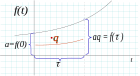
\includegraphics[width=9cm]{allg/funktionen/img/exp/exponentielles_wachstum.png} &
  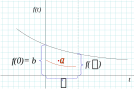
\includegraphics[width=7cm]{allg/funktionen/img/exp/exponentieller_zerfall.png}\\
\end{tabular}

%%\bbwCenterGraphic{10cm}{allg/funktionen/img/exp/exponentieller_zerfall.png}
%%\bbwCenterGraphic{11cm}{allg/funktionen/img/exp/exponentielles_wachstum.png}

Dabei sind
\begin{itemize}
\item $b=f(0)$ der Anfangsbestand zum Zeitpunkt $t$ = 0.
\item $\tau$ ist die typische Zeitspanne zwischen zwei Beobachtungszeitpunkten (zum Beispiel zwischen Wert und dessen Verdopplung). Beispiele:
  \begin{itemize}
  \item Verdoppeln in 3 Stunden: $a=2$ und $\tau = 3\, \text{h}$
    ($\text{h}$ = Stunden)
  \item Verfünf"|fachen einer Viertelstunde (= 15 Minuten): $a=5$ und
    $\tau=\frac{1}{4}\, \text{h}$
  \end{itemize}
  Meist ist die Beobachtungszeit gleichzeitig die Maßeinheit (\zB
  Veränderung pro Stunde). Dann ist unser $\tau=1$ und die Formel
  vereinfacht sich zu $f(t) = b\cdot{}a^t$.
\item $a$ ist der Zunahmefaktor zwischen zwei Beobachtungszeitpunkten (Beispiel $a=2$ bei Verdoppelungsprozessen).
  $a$ berechnet sich durch den Quotienten zwischen zwei
  Beobachtungswerten $a = \frac{f(\tau)}{f(0)} =\frac{m}{b}$.
\item
  Dabei ist $m$ der Messwert zum Zeitpunkt $\tau$.
\item $f(t)=b\cdot{}a^{\frac{t}{\tau}}$ ist der Wert (Anzahl, Fläche,
  Bestand, ...) zum Zeitpunkt
  $t$. 
\end{itemize}

Bemerkung: 
\TNTeop{
$\frac{m}b = \frac{f(\tau)}{f(0)}=\frac{b\cdot{}a^{\frac{\tau}{\tau}}}{b\cdot{}a^{\frac0{\tau}}}
  = \frac{a^1}{a^0} = \frac{a}{1} 
  = a$}%% END TNT
\newpage

\subsection{Referenzaufgabe}\index{Irland!Bevölkerungswachstum}
Irland hatte 1990 3.51 Mio. Einwohner. Im Jahr 2019 waren es bereits 4.93 Mio.

\textbf{Frage 1}: Was prognostizieren Sie für das Jahr 2025, wenn Sie von einem exponentiellen Wachstum ausgehen?

\noTRAINER{\bbwCenterGraphic{12cm}{allg/funktionen/img/exp/IrlandLeer.png}}%%

\TNTeop{
  Skizze:
  \bbwCenterGraphic{12cm}{allg/funktionen/img/exp/IrlandVoll.png}

  $\tau$ = 29 Jahre, Einheit = Jahre ($t$ in Jahren gemessen).
  
  $b=f(0) = 3.51$ [Mio EW] = Startwert (Taschenrechner STO).

  $m=f(\tau) = 4.93$ [Mio EW] = Messwert nach $\tau$ Jahren.

  $a=\frac{m}{b}=\frac{4.93}{3.51} \approx 1.4046$ pro 29 Jahre (Taschenrechner! STO). 

  $$f(t) = b\cdot{}a^\frac{t}{\tau}=b\cdot{}a^\frac{t}{29}$$


  TR Probe $b\cdot{}a^\frac{0}{29} = ? = 3.51$ 

  TR Probe $b\cdot{}a^\frac{29}{29} = ? = 4.93$ 

  Jahr 2025: $t=35$:

    $$f(35) = b\cdot{}a^\frac{35}{29}\approx 5.28899$$

}%% END TNT
\newpage

\subsection*{Aufgaben}

\GESO{\olatLinkArbeitsblatt{Exponentialfunktionen}{https://olat.bms-w.ch/auth/RepositoryEntry/6029794/CourseNode/106029175831971}{Kap. 1.5: Aufg. 18. a) b)}}
\TALS{\olatLinkArbeitsblatt{Exponentialfunktionen}{https://olat.bms-w.ch/auth/RepositoryEntry/6029786/CourseNode/106029175777725}{Kap. 1.5: Aufg. 18. a) b) }}

\newpage

\textbf{Frage 2}: In wie vielen Jahren hat sich die Bevölkerung verdreifacht?

\TNTeop{
  Gesucht $T_3$ = Verdreifachungszeitpunkt.

  $$f(T_3) = 3\cdot{}f(0)$$

  Funktionsgleichung einsetzen:

  $$b\cdot{}a^\frac{T_3}{\tau} = 3\cdot{} b\cdot{} a^\frac0\tau$$

  Weil $a^{\frac{0}{\tau}} = 1$ folgt:

  $$b\cdot{}a^\frac{T_3}{\tau} = 3\cdot{} b$$

  $$a^\frac{T_3}{\tau} = 3$$

  Def. Logarithmus:

  $$\frac{T_3}{\tau} = \log_a(3)$$

$$T_3 = \tau\cdot{}\log_a(3) = 29\cdot{}\log_{\left(\frac{4.93}{3.51}\right)}(3) \approx 93.8$$
Die Bevölkerung wird sich voraussichtlich alle 94 Jahren
verdreifachen.

}%% END Trainer
\newpage

\subsection*{Aufgaben}
%%\TALSAadBMTA{221ff}{831 - 839}


\GESO{\olatLinkArbeitsblatt{Exponentialfunktionen}{https://olat.bms-w.ch/auth/RepositoryEntry/6029794/CourseNode/106029175831971}{Kap. 1.5:
    Aufg. 18. c), 19. - 21.}}
\TALS{\olatLinkArbeitsblatt{Exponentialfunktionen}{https://olat.bms-w.ch/auth/RepositoryEntry/6029786/CourseNode/106029175777725}{Kap. 1.5:
    Aufg. 18. c), 19. - 21. }}

\AadBMTA{338}{28. Bakterien}
\AadBMTA{352ff}{2. (Hasenpopulation), 7., 1. (optional)}
\olatLinkGESOKompendium{3.4}{27ff}{32., 34., 38., 40., 44., 45. und 46.}
\GESO{\aufgabenFarbe{Nullserie 2: Aufgabe 8.}}
\GESO{\aufgabenFarbe{Maturaprüfung 2017, Aufg. 12 (Raupen)\\
Maturaprüfung 2018 (Serie 3), Aufg. 11 (Müll)
}}



%% TODO Arbeitsblatt verlinken
%%\GESO{\olatLinkArbeitsblatt{Exponentialfunktionen}{https://olat.bms-w.ch/auth/RepositoryEntry/6029794/CourseNode/106029175831971}{Kap. 1.1: Voraussetzungen}}
%%\TALS{\olatLinkArbeitsblatt{Exponentialfunktionen}{https://olat.bms-w.ch/auth/RepositoryEntry/6029786/CourseNode/106029175777725}{Kap. 1.1: Voraussetzungen}}



\newpage

\subsection{Rate vs. Faktor
  II}\index{Rate}\index{Fatkor}\index{Zunahmefaktor}\index{Zunahmerate}
\totalref{RateZins1}

Den Unterschied von Zinsfuß (= Rate) und Zinsfaktor kennen wir bereits aus der Zinsrechnung.

So entspricht eine Zunahme von 12\% einem\\
Aufzinsungsfaktor von \LoesungsRaumLang{1.12}.

Wenn jedoch eine Beobachtung einer Zunahme von, sagen wir, 70\% innerhalb einer Viertelstunde beobachtet wird, so können wir uns fragen, um wie viel die Zunahme (als Rate oder Faktor) pro Zeiteinheit (hier Stunden) ist.


Füllen Sie dazu folgende Tabelle aus. Dabei bedeuten

\begin{tabular}{lp{14cm}}\hline
  Einheit & Stunden, Minuten, Meter, ... \\\hline
  $\tau$  & In dieser Zeitspanne (Stunden, Meter, ...) wird beobachtet \\\hline
  $p$     & Zunahme\textbf{rate}\index{Zunahmerate}\index{Rate} während $\tau$ Einheiten in \%. Ist $p$ negativ, handelt es sich um eine Abnahme\\\hline
  $a_\tau$ & Zunahme\textbf{faktor}\index{Zunahmefaktor} während $\tau$ Einheiten. Ist $a<1$, handelt es sich um einen Abnahmefaktor\\\hline
  $a_E$ (Formel)   & Zunahme pro Einheit (als Faktor). Aufgeschrieben als Formel\\\hline
  $\approx a_E$ (Zahl)  & Zunahme pro Einheit (als Näherungswert).\\\hline
  $p_E$   & Prozentuale Zunahme pro Zeiteinheit\\\hline
  \end{tabular} 

\leserluft{}
\leserluft{}
%% temporäres Platzhalterchen 
\newcommand{\ph}[1]{\noTRAINER{...........}\TRAINER{#1}}

%%\renewcommand{\arraystretch}{1.7}
$$f(t) = a_\tau^{\frac{t}\tau} = a_E^t$$
%% probably turn off auto-fill-mode in emacs when editing long lines
\begin{bbwFillInTabular}{|l|l|l|l|l|l|l|}\hline
  Einheit & $\tau$            &  $p$         & $a_\tau$         & $a_E$ (Formel)           &  $\approx a_E$    &$p_E$            \\\hline\hline
  h       &  $3$              &  56\%        & $1.56$           & $1.56^\frac13$            &  1.1598           & 11.598\%        \\\hline 
  h       &  $\frac14 = 0.25$ &  70\%        & \ph{1.7}         & \ph{ $1.7^\frac1{0.25}$}  &  \ph{8.3521}      & \ph{735.21\%}   \\\hline 
  h       &  $\frac12$        &  \ph{50\%}   & 1.5              &  $1.5^\frac1{0.5}$        &  2.25             & \ph{125\%}      \\\hline 
  Tage    &  $5$              & 100\%        & \ph{2}           & \ph{$2^\frac1{5}$}        &  \ph{1.1487}      & \ph{14.87}\%    \\\hline 
  Min.    &  $2$              & \ph{-60}\%   & 0.4              & \ph{$0.4^\frac1{2}$}      &  \ph{0.6325}      & \ph{-36.75}\%   \\\hline 
  m       &  $12$             & \ph{4.5}\%   & \ph{1.045}       & $1.045^\frac1{12}$        &  \ph{1.00367}     & \ph{0.3675}\%   \\\hline
  Wochen  & \ph{$2$}          & \ph{$200$}\% & \ph{3}           & $3^\frac12$               & \ph{1.73205}      & \ph{73.205}\%   \\\hline
  Jahr    & \ph{$\frac1{12}$} & \ph{$1$}\%   & \ph{$1.01$}      & $1.01^{\frac1{1/12}}$      &  \ph{$1.127$}     & \ph{$12.7$}\%   \\\hline
\end{bbwFillInTabular} 

\newpage

\subsection{Basistransformtaionen\GESO{ (optional)}}
Die Algen (im Türlersee) verdoppeln sich alle fünf Tage.

$$\tau = 5; a= 2$$

Die Exponentialfunktion bei Startwert $b$ lautet also:

\TNT{2.4}{$$f(t) = b\cdot{} 2^\frac{t}5 \left(\stackrel{!}{=} b\cdot{} 4^{\frac{t}{10}}\right)$$}


Um wie viel nehmen sie ...

\begin{enumerate}
\item ... alle 15 Tage zu?
\item ... alle 7 Tage zu?
\item In wie vielen Tagen verdreifachen sie sich?
\end{enumerate}
\subsubsection{Natürliche Basen}

\begin{enumerate}[resume]
\item Wie viel nehmen die Algen pro Tag (= pro (Zeit)einheit) zu?
\item \GESO{(optional) }Wie sieht es mit der Basis $\e$ aus? Mit welchem $m$ kann man die
  Zunahme als $f(t) = b \cdot{} \e^{m\cdot{}t}$ angeben?
\end{enumerate}
\newpage


\subsubsection*{Lösungen...}

Zu Punkt 1.: «Um wie viel nehmen sie alle 15 Tag zu?» $\tau_2=15$:

\TNT{4}{

  $2^\frac15 = a_2^\frac1{15}$ Nun auf beiden Seiten ``hoch
  15'' und somit

  $a_2 = (2^{\frac15})^{15} = 2^3 = 8$.

Ergo $b\cdot{}2^\frac{t}5 = b\cdot{} 8^\frac{t}{15}$}

Zu Punkt 2.: «Um wie viel nehmen sie alle 7 Tage zu?» $\tau_2=7$:

\TNT{4}{

  $2^\frac15 = a_2^\frac1{7}$ Nun auf beiden Seiten ``hoch
  7'' und somit

  $a_2 = (2^{\frac15})^{7} = 2^{\frac75} \approx 2.639$.

Ergo $b\cdot{}2^\frac{t}5 \approx b\cdot{} 2.639^\frac{t}{7}$}

Zu Punkt 3.: «In wie vielen Tagen verdreifachen sie sich?» $a_2 = 3$
(verdreifachen):

\TNTeop{
  $$f(t) = b\cdot{} 2^{\frac{t}{5}}$$
  
$$f(0)\cdot{} 3 = f(\tau_3)$$

  $$b\cdot{}3 = b\cdot{} 2^{\frac{\tau_3}{5}}$$

  $$3 =2^{\frac{\tau_3}{5}}$$

  $$3^5 =2^{\tau_3}$$

  $$\tau_3 = \log_2{3^5} \approx 7.925$$
  
Also: Sie verdreifachen sich ca. alle 8 Tage.

  Ergo: $b\cdot{}2^\frac{t}5 \approx b\cdot{}3^\frac{t}{7.925}$
}%% end TNT
\newpage


\subsubsection*{... natürliche Basen}
Zu Punkt 4.: «Wie viel nehmen die Algen pro Tag (= pro Zeiteinheit) zu?»
\TNT{5.6}{

  Generell: $f(t) = b\cdot{} A^t$ mit $A$ = Zunahme pro Zeiteinheit (hier
  pro Tag)

  Ansatz:
  $$2\cdot{} f(0) = f(5)$$

  Einsetzen:
  $$2\cdot{} b\cdot{}A^0 = b\cdot{} A^5$$
  $$2 = A^5 | \sqrt[5]{\,}$$
  $$A = \sqrt[5]{2} = 2^{\frac15} \approx 1.1487$$
  ergo
  $$f(t) = b\cdot{} \left( 2^\frac15 \right)^t \approx b\cdot{} 1.1487^t$$
}%% END TNT

Zu Punkt 5.\GESO{ (optional)}: »Wie sieht es mit der Basis $\e$ aus?» $f(t) = b\cdot{}\e^{m\cdot{}t}$ (Basis $\e$):
\TNTeop{

  
  Auch hier Ansatz:
 
$$2\cdot{} f(0) = f(5)$$
  Funktionsterm einsetzen:
  $$2 \cdot{} b\cdot{} e^{m\cdot{} 0} = b\cdot{} e^{m\cdot{} 5}$$

  $$2 = e^{m\cdot{}5}$$
  Beidseitig logarithmieren ($\ln$):
  $$\ln(2) = m \cdot{} 5$$
  $$m = \frac{\ln(2)}{5} \approx 0.1386$$

  Somit lautet die Funktion:
  $$f(t) \approx  b\cdot{} e^{0.1386\cdot{} t}$$
  
  Bedeutung: Gerade $g(t): y=0.1386\cdot{}t+b$ zeichnen: Dies ist die
  Tangente an die Exponentialfunktion $b\cdot{}2^\frac{t}{5} = b\cdot{}4^\frac{t}{10}$
}%% END TNT
\newpage

\subsection*{Aufgaben}
%%\TALSAadBMTA{215ff}{809-830}
\AadBMTA{335ff}{17. a) b) d), 22. a)}

\newpage
\subsubsection{Zusammenfassung\GESO{ (optional)}}
\begin{center}\fbox{
    \textbf{ $\tau$ und $a$ sind voneinander abhängig!}}
  \end{center}

\begin{beispiel}{Basiswechsel}{}
  Warum ist $$b\cdot{}2^{\frac{t}7} = b \cdot{} 8^{\frac{t}{21}}$$
  \TNT{1.2}{Lösung: 2x in 7h = 4x in 14 h = 8x in 21 h}
\end{beispiel}


\begin{gesetz}{Basiswechsel}{}

  \begin{center}\fbox{\fbox{
          $a^{\frac{1}{\tau}} =
        \LoesungsRaumLen{30mm}{a_2^{\frac{1}{\tau_2}}}
        \TALS{ = \LoesungsRaumLen{30mm}{\e^{m}}}$
    }}
  \end{center}

 
  $a=$ Wachstumsfaktor\\
  $b=$ Startwert\\
  $\tau=$ Beobachtungszeitraum\\

  Basis $a$ zum Beobachtungsintervall $\tau$:
  $$y = b\cdot{} a^{\frac{t}\tau}$$

  Natürliche Basis $A$ zur (Zeit)Einheit:

  $$y = \LoesungsRaumLen{30mm}{b\cdot{}A^t}$$
  mit $$A=\LoesungsRaumLen{30mm}{a^{\frac1\tau} = \sqrt[\tau]{a}}$$

  \TALS{
    Natürliche Basis $\e\,\, (=2.718...)$:

    $$y=\LoesungsRaumLen{30mm}{b\cdot{}e^{mt}}$$
mit $$m=\LoesungsRaumLen{30mm}{\frac{\ln(a)}{\tau}}$$
    

    $m = $ \textit{Wachstumsexponent} bei Basis $e$ \\
 }%% end TALS
\end{gesetz}
\newpage


\subsection{Halbwertszeit, Verdopplungszeit}\index{Halbwertszeit}\index{Verdopplungszeit}

\begin{definition}{Halbwertszeit}{}
Die Zeitspanne, in der sich ein Wert bei exponentiellem Zerfall halbiert, nennen wir
\textbf{Halbwertszeit} und bezeichnen diese Zeit mit:

$$T_{1/2}$$
Ansatz:
$$\frac12 \cdot{} f(0) = f(T_{1/2})$$
\end{definition}

Die Halbwertszeit wird insbesondere
  beim radioaktiven Zerfall verwendet. Typische Frage: Nach wie viel
  Jahren strahlt ein Stoff nur noch die Hälfte?
\hrule
Beispiel: Ein Stoff nimmt innerhalb von sieben Tagen auf 80\% ab. Wie
groß ist seine Halbwertszeit $T_{1/2}$?

\noTRAINER{\bbwCenterGraphic{85mm}{allg/funktionen/img/exp/HalbwertszeitLeer.png}}
  \TRAINER{\bbwCenterGraphic{75mm}{allg/funktionen/img/exp/Halbwertszeit.png}}

\TNTeop{
  
  Ansatz «halber Wert»: $\frac12\cdot{}f(0) = f(T_{1/2})$.

  Funktionsgleichung $f(t) = b\cdot{} a^{\frac{t}\tau}$ einsetzen

  $$\frac12 \cdot{} b\cdot{} a^{\frac0\tau} = b\cdot{} a^{\frac{T_{1/2}}{\tau}}$$

  Vereinfachen
  $$\frac12 = a^{\frac{T_{1/2}}{\tau}} \stackrel{\log}{\Longrightarrow}  \log_a\left(\frac12\right) = \frac{T_{1/2}}{\tau}$$

  $$\Longrightarrow T_{1/2} = \tau \cdot{} \log_a\left(\frac12\right)$$
  
  $80\%$ und $7$ Tage einsetzen:

  $$T_{1/2} = 7 \cdot{} \log_{0.8}\left(\frac12\right) \approx 21.74$$
    
%%  Bemerkung: $$f(t) =b\cdot{}0.8^\frac{t}7 \approx b\cdot{}\left(\frac12\right)^\frac{t}{21.74}$$

}%% END TNTeop



\begin{gesetz}{Halbwertszeit}{}
  Die Halbwertszeit $T_{1/2}$ berechnet sich wie folgt:
  $$T_{1/2} = \LoesungsRaumLen{70mm}{\tau \cdot{} \log_a\left(\frac12\right)}$$
  Dabei ist $a$ der Abnahmefaktor pro Zeiteinheit $\tau$.
\end{gesetz}

Ist die Halbwertszeit $T = T_{1/2}$ bekannt, so gilt mit
$\tau=T_{1/2}$ und mit $a=\frac12$:

\begin{gesetz}{Stoffmenge}{}
  Ist die Halbwertszeit $T_{1/2}$ und die anfängliche Stoffmenge $b$
  bekannt, so kann die Stoffmenge zu jedem Zeitpunkt $t$ mit der
  folgenden Funktion $f$ angegeben werden:
  \leserluft{}
  \leserluft{}  
  $$f(t) = \LoesungsRaumLen{50mm}{b\cdot{}\left(\frac12\right)^{\frac{t}{T_{1/2}}}}$$
\end{gesetz}
  
\newpage
\GESO{Optional:}

\subsection{Verdopplungszeit}\index{Verdopplungszeit|textbf}

Analog gilt das Gesetz zur Verdopplung (s. obiges Beispiel Bevölkerung Irlands):
\begin{gesetz}{Verdopplungszeit}{}
  $$T_2 = \LoesungsRaumLen{40mm}{ \tau \cdot{} \log_a(2)}$$

  $a$: Zunahmefaktor pro Zeiteinheit $\tau$.
\end{gesetz}

(optional:)

\begin{bemerkung}{Verdopplungszeit}{}
  Ansatz:$$2 \cdot{} f(0) = f(T_2)$$
  Funktionsterm einsetzen:
  %%  $$2 \cdot{} b \cdot{} a^{\frac{0)\tau} = b \cdot{} a^{\frac{T_2}\tau}$$
  $$2 \cdot{} b \cdot{} a^{\frac{0}{\tau}} = b \cdot{} a^{\frac{T_2}{\tau}}$$
    $$2 = a^{\frac{T_2}\tau} \Longrightarrow  T_2 = \tau \cdot{} \log_a(2)$$
\end{bemerkung}


%\begin{gesetz}{Vervielfachungszeit $T_q$}{}
%  Die Vervielfachungszeit $T_q$ kann durch die Vervielfachung $q$ ausgedrückt werden. Es gilt:
%  $$T_q = \tau\cdot{}\log_a(q)$$
%  und
%  $$f(t) = b\cdot{} q^{\frac{t}{T_q}}$$
%  \end{gesetz}

\subsection*{Aufgaben}

\GESO{\olatLinkArbeitsblatt{Exponentialfunktionen}{https://olat.bms-w.ch/auth/RepositoryEntry/6029794/CourseNode/106029175831971}{Kap. 1.6:
    Halbwertszeit/Verdopplungszeit: Aufg. 22. - 25.}}
\TALS{\olatLinkArbeitsblatt{Exponentialfunktionen}{https://olat.bms-w.ch/auth/RepositoryEntry/6029786/CourseNode/106029175777725}{Kap. 1.6:
    Halbwertszeit/Verdopplungszeit: Aufg. 22. - 25.}}

\AadBMTA{352ff}{3. (Taucherin), 4. [Glasfaser ohne Teilaufgabe
    Eindringtiefe 4. b)] und 5. b) (radioaktiver Zerfall)}

\olatLinkGESOKompendium{3.4}{28ff}{42., 43. und 47.}

\GESO{\aufgabenFarbe{
    Maturaprüfung 2020, Aufg 11 (Käfer)\\
    Maturaprüfung 2018 (Serie 4), Aufg 10 (Cäsium 137)\\
    Maturaprüfung 2018 (Serie 2), Aufg 11 (Plutonium)\\
    Maturaprüfung 2018 (Serie 1), Aufg 11 (radioaktive Substanz)\\
    Maturaprüfung 2016, Aufg. 9 (Jod-131)
}}

\olatLinkGESOKompendium{3.4}{27ff}{32. bis 47.}

\newpage
